\documentclass[compress]{beamer}
\usepackage{ifthen,verbatim,ulem}

\newcommand{\isnote}{}
\xdefinecolor{lightyellow}{rgb}{1.,1.,0.25}
\xdefinecolor{darkblue}{rgb}{0.1,0.1,0.7}

%% Uncomment this to get annotations
%% \def\notes{\addtocounter{page}{-1}
%%            \renewcommand{\isnote}{*}
%% 	   \beamertemplateshadingbackground{lightyellow}{white}
%%            \begin{frame}
%%            \frametitle{Notes for the previous page (page \insertpagenumber)}
%%            \itemize}
%% \def\endnotes{\enditemize
%% 	      \end{frame}
%%               \beamertemplateshadingbackground{white}{white}
%%               \renewcommand{\isnote}{}}

%% Uncomment this to not get annotations
\def\notes{\comment}
\def\endnotes{\endcomment}

\setbeamertemplate{navigation symbols}{}
\setbeamertemplate{headline}{\mbox{ } \hfill
\begin{minipage}{5.5 cm}
\vspace{-0.75 cm} \small
\end{minipage} \hfill
\begin{minipage}{4.5 cm}
\vspace{-0.75 cm} \small
\begin{flushright}
\ifthenelse{\equal{\insertpagenumber}{1}}{}{Jim Pivarski \hspace{0.2 cm} \insertpagenumber\isnote/\pageref{numpages}}
\end{flushright}
\end{minipage}\mbox{\hspace{0.2 cm}}\includegraphics[height=1 cm]{../cmslogo} \hspace{0.1 cm} \includegraphics[height=1 cm]{../tamulogo} \hspace{0.01 cm} \vspace{-1.05 cm}}

\begin{document}
\begin{frame}
\vfill
\begin{center}
\textcolor{darkblue}{\Large Shape of the DT Chambers \\ \vspace{0.2 cm} from Track-based Studies}

\vfill
\begin{columns}
\column{0.3\linewidth}
\begin{center}
\large
\textcolor{darkblue}{Jim Pivarski}

\vspace{0.2 cm}
Alexei Safonov
\end{center}
\end{columns}

\begin{columns}
\column{0.3\linewidth}
\begin{center}
\scriptsize
{\it Texas A\&M University}
\end{center}
\end{columns}

\vfill
28 January, 2009

\end{center}
\end{frame}

%% \begin{notes}
%% \item This is the annotated version of my talk.
%% \item If you want the version that I am presenting, download the one
%% labeled ``slides'' on Indico (or just ignore these yellow pages).
%% \item The annotated version is provided for extra detail and a written
%% record of comments that I intend to make orally.
%% \item Yellow notes refer to the content on the {\it previous} page.
%% \item All other slides are identical for the two versions.
%% \end{notes}

\small

\begin{frame}
\frametitle{The clue (\only<1>{1}\only<2>{2}\only<3>{3}/3)}

\only<1>{\includegraphics[height=\linewidth, angle=90]{DTrphiVsPhi_st1_whB.pdf}}
\only<2>{\includegraphics[height=\linewidth, angle=90]{DTrphiVsPhi_st1_whC.pdf}}
\only<3>{\includegraphics[height=\linewidth, angle=90]{DTrphiVsPhi_st1_whD.pdf}}

\vspace{-0.5 cm}
\only<1>{\begin{itemize}
\item Linear trends in unbiased $r\phi$ residual vs.\ $\phi$ inside each chamber
\item Unaffected by local $x$ alignment (as expected)
\item Curious thing: they all seem to have the same slope
\end{itemize}}
\only<2>{\begin{itemize}
\item What if it's a linear bias in the distribution from the track source, partly absorbed by the alignment?
\begin{itemize}
\item impossible: $\phi$ must have periodic boundary conditions
\item if we realigned chambers to make a continuous line, it could not match at $\pm\pi$ (it would fail a ``closure condition'')
\end{itemize}
\end{itemize}}
\only<3>{\begin{itemize}
\item So it's a real effect related to the chambers, not the track source
\begin{itemize}
\item not fixing it would smear chamber resolution by 5~mm!
\end{itemize}
\item What rigid body misalignments can cause it?
\begin{itemize}
\item $\phi_y$ (rotation around axis parallel to the beamline)
\item $\Delta R$ (radial displacements)
\end{itemize}
\end{itemize}}
%% \hspace{-0.83 cm} \textcolor{darkblue}{\Large Outline2}
\end{frame}

\begin{frame}
\frametitle{The $\phi_y$ possibility}

\begin{columns}
\column{0.5\linewidth}
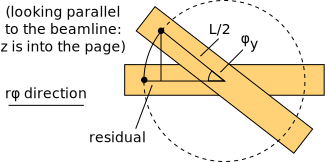
\includegraphics[width=\linewidth]{phiy_explanation.png}

\column{0.5\linewidth}
\begin{itemize}
\item $\phi_y$ rotation can make a chamber appear narrower
\item but it's a second-order effect:
\end{itemize}

\vspace{-0.75 cm}
\begin{eqnarray*}
\mbox{residual} &=& (L/2) \left(1 - \cos\phi_y\right) \\
\phi_y &\approx& \mbox{70~mrad}
\end{eqnarray*}
\end{columns}

\vfill
\begin{itemize}
\item Could {\it all} the chambers be independently misaligned by about 70~mrad?
\item Same effect observed in IDEAL and CRAFT\_ALL\_V4 constants: it
  would have to be a physical misalignment of real chambers
\item I think we can safely say that this is not what's happening
\begin{itemize}
\item the magnitude is too big, and
\item the pattern is too regular
\end{itemize}
\end{itemize}
\end{frame}

\begin{frame}
\frametitle{The $\Delta R$ possibility}

\begin{columns}
\column{0.7\linewidth}
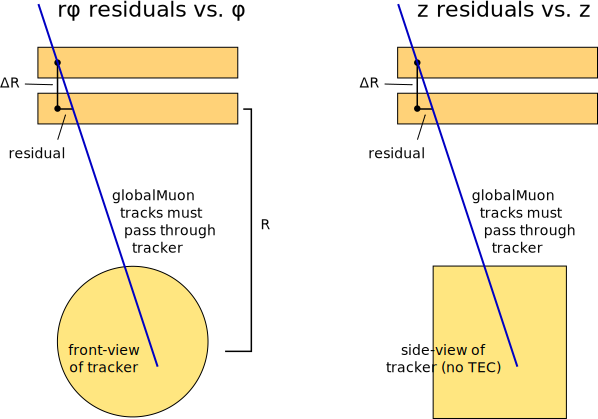
\includegraphics[width=\linewidth]{z_explanation.png}

\column{0.3\linewidth}
\begin{itemize}
\item A track sample constrained to pass through the tracker can introduce effects of this sort

\vspace{0.2 cm}
\mbox{\hspace{-1 cm}$\displaystyle \Delta R = \frac{R}{(L/2)} \left(\mbox{residual}\right)$\hspace{-1 cm}}

\vspace{0.1 cm}
\item But it has to appear in both types of residuals
\end{itemize}
\end{columns}
\end{frame}

\begin{frame}
\frametitle{Trial $\Delta R$ alignment (1/2)}

\begin{itemize}
\item To see if this is plausible, I expanded the radius of all DT stations by 15~mm in a private test
\begin{itemize}
\item seems to cancel the $r\phi$ residual vs.\ $\phi$ trend in the $-\pi < \phi < 0$ range, but overshoot slightly in the $0 < \phi < +\pi$ range
\end{itemize}
\end{itemize}

\includegraphics[height=\linewidth, angle=90]{DTrphiVsPhi_st1_whC_out15mm.pdf}
\end{frame}

\begin{frame}
\frametitle{Trial $\Delta R$ alignment (2/2)}

\begin{itemize}
\item However, look what happens to the $z$ residual vs.\ $z$: clearly both types of residuals can't be satisfied!
\item The open circles are the case of no $\Delta R$ shift
\end{itemize}

\includegraphics[height=\linewidth, angle=90]{DTzVsZ_st1_sr02_out15mm.pdf}
\end{frame}

\begin{frame}
\frametitle{So, what could it be?}

\begin{itemize}
\item Process of elimination for all rigid body degrees of freedom

\begin{itemize}
\item \sout{$\phi_y$: implausible}
\item \sout{$\Delta R$ (a local $z$ translation): can't reconcile both $r\phi$ and $z$ residuals}
\item local $x$, $y$ translations: can't introduce any linear trends in residuals, only offsets
\item $\phi_z$ rotation: introduces a linear trend in $r\phi$
  residuals vs.\ $z$ and $z$ residuals vs.\ $\phi$, but not what we're
  looking for
\item $\phi_x$ rotation: also would have to be implausibly large, and only affects $z$ residuals (the opposite of what we're looking for)
\end{itemize}

\item Non-rigid degree of freedom \hfill 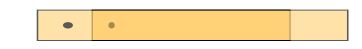
\includegraphics[width=0.35\linewidth]{stretch_explanation.png}

\begin{itemize}
\item {\it some kind} of stretching would easily explain it
\item an error in the geometry description, duplicated by CMSSW, would
  account for its regularity (with outliers due to small individual
  $\Delta R$ misalignments)
\end{itemize}
\end{itemize}
\end{frame}

\begin{frame}
\frametitle{Regularity of the effect}
\includegraphics[width=\linewidth]{slopehist.png}

\begin{itemize}
\item Distribution of slopes in $r\phi$ residuals vs.\ $\phi$ (wheels
  $-$1, 0, $+$1) \\ peaks at roughly 10~mm/radian
\item 0 underflows, 1 overflow
\item Small individual $\Delta R$ misalignments can smear this
\end{itemize}
\end{frame}

\begin{frame}
\frametitle{Analogy with CSC case}
\begin{itemize}
\item Last year, a similar track-based technique uncovered a 0.8~mm error in CSC widths
\item For the same reasons, chamber stretching was degenerate with increasing the distance from the beamline
\item Degeneracy was resolved with photogrammetry of alignment pins
\begin{itemize}
\item track-based procedure reproduced $r\phi$ positions of alignment pins with 270~$\mu$m accuracy
\item $R$ positions of pins were therefore directly comparable, and constrained distance from the beamline
\end{itemize}
\item CSC geometry experts investigated and quickly found a 10~$\mu$m strip pitch
  angle error, which, compounded over 80~strips, changed the width by
  0.8~mm, explaining the observation with tracks
\item DTs have an advantage over CSCs in that they precisely measure
  $z$ residuals in addition to $r\phi$ residuals, so we can already
  break degeneracy between $\Delta R$ and stretching
\item In the CSC case, we predicted the magnitude but made a mistake in guessing
  the sign: we'd follow up on any effect of this magnitude
\end{itemize}
\end{frame}

%% \section*{First section}
%% \begin{frame}
%% \begin{center}
%% \Huge \textcolor{blue}{First section}
%% \end{center}
%% \end{frame}

\begin{frame}
\frametitle{Conclusions: what to do?}
\begin{itemize}\setlength{\itemsep}{0.2 cm}
\item I would like to ask DT geometry experts to look for a chamber
  description error on the order of 5~mm across the local $x$
  dimension

\item We have shown that it is a real chamber-level effect and ruled
  out the possibility of it being caused by any rigid chamber misalignment

\item ``Stretching/squashing'' can be interpreted loosely
\begin{itemize}
\item only distortions which affect active elements matter
\item a bulging layer can look narrow (though that's a second-order effect, like $\phi_y$)
\item a $\phi_y$ $\sim$ 70~mrad rotation built into the chamber?
\item a $\Delta R$ misalignment for superlayers 1 and 3 and not superlayer 2 could explain the incompatibility of $r\phi$ and $z$ residuals
\item it's hard to imagine timing effects playing a role, since left- and right-hand sides of each wire would be affected oppositely
\item \ldots
\end{itemize}

\item Since it's causing $\pm 2.5$~mm unbiased residuals errors at the ends of
  the chambers, it's as important for resolution as alignment

\end{itemize}
\label{numpages}
\end{frame}

\end{document}
